\let\negmedspace\undefined
\let\negthickspace\undefined
\documentclass[journal,12pt,twocolumn]{IEEEtran}
\usepackage{cite}
\usepackage{amsmath,amssymb,amsfonts,amsthm}
\usepackage{algorithmic}
\usepackage{graphicx}
\usepackage{textcomp}
\usepackage{xcolor}
\usepackage{txfonts}
\usepackage{listings}
\usepackage{enumitem}
\usepackage{mathtools}
\usepackage{gensymb}
\usepackage[breaklinks=true]{hyperref}
\usepackage{tkz-euclide} % loads  TikZ and tkz-base
\usepackage{listings}
\usepackage{geometry}

\geometry{margin=1in}

% correct bad hyphenation here
\hyphenation{op-tical net-works semi-conduc-tor}
\def\inputGnumericTable{}       

\lstset{
%language=C,
frame=single, 
breaklines=true,
columns=fullflexible
}

\begin{document}

\vspace{3cm}

\title{Music Player Code Report - AI1110}
\author{Nimai Parsa}

\maketitle

\section{Introduction}
This report provides an overview and analysis of the Python code for a music player implemented using the Tkinter and Pygame Modules. It also includes a song shuffling function.

\section{Code Explanation}
\subsection{Music Player}
\begin{itemize}
  \item The code starts by importing the necessary modules: Tkinter and Pygame.
  \item It initializes the Pygame mixer using \texttt{mixer.init()}.
  \item The \texttt{playSong()} function is defined to play a song. It checks the index of the song in the \texttt{songShuffler} module and loads and plays the corresponding song using the Pygame mixer.
  \item The code then creates a GUI using Tkinter. It creates a window titled "Music Player" with a fixed size.
  \item Several buttons are defined: "play", "next", "stop", "pause", and "resume". These buttons are associated with specific commands to control the music playback using the Pygame mixer functions.
  \item The "song" label displays the current song playing in the music player.
  \item The GUI layout is organized using the grid system, and the buttons are placed in different rows and columns within the root window.
  \item Finally, the GUI is updated and the main event loop is started using \texttt{root.update()} and \texttt{root.mainloop()}.
\end{itemize}

\subsection{Randomizer}
\begin{itemize}
  \item The function takes two arguments, \texttt{start} and \texttt{end}, representing the range of numbers to be shuffled.
  \item It initializes an array called \texttt{songs} with \texttt{None} values to store the shuffled songs.
  \item A separate array called \texttt{visited} is initialized to keep track of which numbers have been visited.
  \item The function uses a while loop to generate a random song number between \texttt{start} and \texttt{end} (inclusive).
  \item It checks if the generated song number has already been visited. If so, it generates a new random number until an unvisited number is found.
  \item Once an unvisited number is found, it is added to the \texttt{songs} array and marked as visited in the \texttt{visited} array.
  \item The process continues until all the songs have been added to the \texttt{songs} array.
  \item Finally, the shuffled \texttt{songs} array is returned.
\end{itemize}


\section{Output}
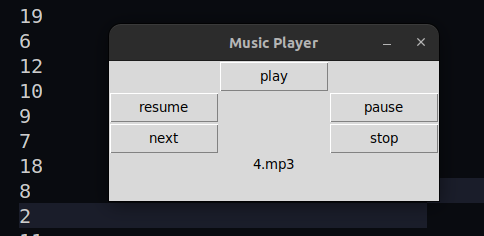
\includegraphics[scale=0.5]{images/Output.png}

\section{Conclusion}
The code provides a basic implementation of a music player using the Tkinter and Pygame libraries in Python. It also includes a song shuffling function that generates a random permutation of numbers within a given range. This function can be used to shuffle the songs played by the music player, adding variety to the playlist.
\end{document}
